%----------------------------------------------------------------------------------------
% METADATA BLOCK (YAML)  — see inbox/README.md
%----------------------------------------------------------------------------------------
% uid: ""
% school: "lycee"
% level: "2eme"
% section: ["Sciences", "Informatique"]
% chapter: "Barycentre"
% title: "Placer des barycentres sur une droite"
% difficulty: "Facile"
% tags: ["barycentre", "deux-points", "construction"]
% provenance: "own"
% batch: "2026-11-19-2sc-polynomes-barycentre"
%----------------------------------------------------------------------------------------

\newcommand{\R}{\mathbb{R}}
\newcommand{\vect}[1]{\overrightarrow{#1}}

% ---STATEMENT---
Soient $A$ et $B$ deux points tels que $AB=6$ cm.
\begin{enumerate}
  \item Construire les points suivants, après avoir exprimé $\vect{AG_k}$ en fonction de $\vect{AB}$ :
  \begin{enumerate}
    \item $G_1$ barycentre de $(A,1)$ et $(B,3)$ ;
    \item $G_2$ barycentre de $(A,2)$ et $(B,-1)$ ;
    \item $G_3$ barycentre de $(A,-1)$ et $(B,3)$ ;
    \item $G_4$ barycentre de $(A,5)$ et $(B,5)$.
  \end{enumerate}
  \item Montrer que $A$ est le barycentre de $(G_1,4)$ et $(B,-3)$.
  \item Montrer que $B$ est le barycentre de $(A,1)$ et $(G_3,2)$.
\end{enumerate}

% ---SOLUTION---
\begin{center}
% alt: Droite (AB) graduée en centimètres avec les points G2, A, G4, G1, B, G3.
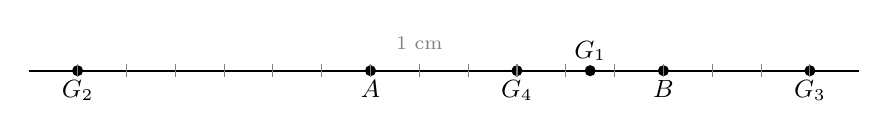
\begin{tikzpicture}[x=0.62cm, font=\small]
  \draw[thick] (-7,0)--(10,0);
  \foreach \p/\v/\pos in {G_2/-6/below, A/0/below, G_4/3/below, G_1/4.5/above, B/6/below, G_3/9/below}
    {\fill (\v,0) circle (2pt) node[\pos] {$\p$};}
  \foreach \v in {-6,...,9} \draw[gray] (\v,0.08)--(\v,-0.08);
  \node[gray] at (1,0.35) {\scriptsize 1 cm};
\end{tikzpicture}
\end{center}
\begin{prop}[Position du barycentre de deux points]
Si $\alpha+\beta\neq0$ et si $G$ est le barycentre de $(A,\alpha)$ et $(B,\beta)$, alors \ib{$\vect{AG}=\dfrac{\beta}{\alpha+\beta}\,\vect{AB}$}.
\end{prop}
\begin{enumerate}[itemsep=14pt]
  \item
  \begin{enumerate}[itemsep=8pt]
    \item $\alpha+\beta=1+3=4\neq0$ :\quad $\vect{AG_1}=\dfrac34\vect{AB}$. \quad $G_1\in[AB]$, à $4{,}5$ cm de $A$.
    \item $\alpha+\beta=2-1=1\neq0$ :\quad $\vect{AG_2}=\dfrac{-1}{1}\vect{AB}=-\vect{AB}$. \quad $G_2$ est le symétrique de $B$ par rapport à $A$.
    \item $\alpha+\beta=-1+3=2\neq0$ :\quad $\vect{AG_3}=\dfrac32\vect{AB}$. \quad $G_3$ est sur la demi-droite $[AB)$, à $9$ cm de $A$ (donc $3$ cm après $B$).
    \item $\alpha+\beta=10\neq0$ :\quad $\vect{AG_4}=\dfrac{5}{10}\vect{AB}=\dfrac12\vect{AB}$. \quad $G_4$ est le milieu de $[AB]$.
  \end{enumerate}
  \textbf{Remarque :} des coefficients égaux donnent toujours le milieu ; des coefficients de signes contraires placent le point \emph{hors} du segment.

  \item
  \begin{prop}[Reconnaître un barycentre]
  Si \ib{$\alpha\vect{GA}+\beta\vect{GB}=\vec0$} avec $\alpha+\beta\neq0$, alors $G$ est le barycentre de $(A,\alpha)$ et $(B,\beta)$.
  \end{prop}
  On part de $\vect{AG_1}=\dfrac34\vect{AB}$ et on multiplie par $4$ :
  \[4\vect{AG_1}=3\vect{AB}\qquad\text{soit}\qquad4\vect{AG_1}-3\vect{AB}=\vec0\]
  C'est une relation écrite \emph{à partir du point $A$}, avec la somme $4+(-3)=1\neq0$ :
  \[\ib{$A$ est le barycentre de $(G_1,4)$ et $(B,-3)$.}\]

  \item On part de $\vect{AG_3}=\dfrac32\vect{AB}$, donc
  \[\vect{AB}=\dfrac23\vect{AG_3}=\dfrac{2}{1+2}\vect{AG_3}\]
  D'après la propriété de position (avec $\alpha=1$ et $\beta=2$) : $B$ est le barycentre de $(A,1)$ et $(G_3,2)$.
\end{enumerate}
